%%% Research Diary - Entry
%%% Template by Mikhail Klassen, April 2013
%%%
\documentclass[11pt,letterpaper]{article}

\usepackage[all]{xy}


\newcommand{\workingDate}{\textsc{2016 $|$ Winter}}
\newcommand{\userName}{Yonsei-HEP-COSMO}
\newcommand{\institution}{Yonsei University}
\usepackage{researchdiary_png}
% To add your univeristy logo to the upper right, simply
% upload a file named "logo.png" using the files menu above.

\begin{document}
\univlogo

\title{QFT Study}

{\Huge \bfseries QFT Study in 2016 Winter}\\[3mm]

\section*{Study Plan}

\subsection*{$-$ Main Text \& References}

Main text book is Peskin \& Schroeder. We will deal with whole examples and final projects in Peskin. \newline
For references, maybe we will use Schwartz, Nair, Zee, Ryder and Maggiore.

\subsection*{$-$ Specific Plan}

\begin{enumerate}[I.]
 \item \textbf{4th week, November - 11/25} \newline
 : Preliminaries of QFT - Motivation of QFT, Klein-Gordon equation \& SHO.
 \item \textbf{5th week, November - 11/29} \newline
 : Group Theory (Lorentz to Poincar\'e), Dirac equation.
 \item \textbf{2nd week, December - 12/04, 12/06, 12/09} \newline
 : Canonical Quantization of KG \& Dirac Field, Weyl \& Majorana Spinors, Majorana mass.
 \item \textbf{1st week, January - 1/4, 1/8} \newline
 : Review of Spinor Fields.
 \item \textbf{2nd week, January - 1/11} \newline
 : Introduce Path integral formalism.
 \item \textbf{3rd week, January - 1/17, 1/20} \newline
 : Cross section, LSZ reduction, Perturbative Expansion and Feynman Rule.
 \item \textbf{4th week, January - 1/23, 1/26} \newline
 : Renormalization \& Quantum Electrodynamics.
 \item \textbf{1st week, Feburary - 1/31, 2/3} \newline
 : Rest of Path integral formalism and Renomalization \& Implication of Unitarity.
 \item \textbf{2nd week, Feburary - 2/6, 2/10} \newline
 : Non-abelian gauge theory, Spontaneous symmetry breaking \& Weak interaction.
 \item \textbf{3rd week, Feburary - 2/13, 2/17} \newline
 : HEP tools (CalcHEP, Madgraph, Feynrules)
 \item \textbf{2nd week, Feburary - 2/20, 2/24} \newline
 : Quantum Yang-Mills Theory
\end{enumerate}

\newpage

\section*{The Limit of NRQM}

\subsection*{1. Causality Violation}

\subsubsection*{1) Classical Hamiltonian : $H=\dfrac{P^2}{2m}$}

Consider the transitional amplitude - $U(t,x;0,x_0) \equiv \braket{x,t|x_0,0} = \TA{x}{Ht}{x_0}$

\begin{equation}
 \begin{split}
  U(t,x;0,x_0) &= \TA{x}{\tfrac{P^2}{2m}t}{x_0} = \Ip \TA{x}{\tfrac{P^2}{2m}t}{p}\braket{p|x_0} =
  \frac{1}{(2\pi)^3}\Ip e^{-i \tfrac{\vp^2}{2m}t}\ld e^{i\vp\cdot (\vec{x}-\vec{x_0})}  \\
               &= \frac{1}{(2\pi)^3}\Ip e^{-\tfrac{it}{2m}\BKS{\vp-\tfrac{m(\vec{x}-\vec{x_0})}{t}}^2}
  e^{i\tfrac{m}{2t}(\vec{x}-\vec{x_0})^2} = \BKS{\frac{m}{2\pi it}}^{\frac{3}{2}}e^{\tfrac{im}{2t}(\vec{x}-\vec{x_0})^2}
 \end{split}
\end{equation}

$\therefore$ Since, this expression is nonzero for all $x, t$, indicating that a particle can propagate between any
two points in an arbitrarily short time. $\Rightarrow$ Causality violation.

\VS

\subsubsection*{2) Relativistic Hamiltonian : $H = \sqrt{\left|\vp\right|^2 + m^2}$}

\begin{equation}
 \begin{split}
  U(t,x;0,x_0) &= \Ip \TA{x}{\sqrt{\left|\vp\right|^2 + m^2}}{p}\braket{p|x_0} \\
               &= \int \frac{dp}{(2\pi)^3}(2\pi)\avp^2 e^{-it\sqrt{\avp^2 + m^2}} \int_0^\pi d\theta\sin{\theta} \hs e^{i\avp\abs{\vec{x}-\vec{x_0}}\cos{\theta}} \\
               &= \frac{1}{2\pi^2}\int dp \avp\sin(\avp\abs{\vec{x}-\vec{x_0}})e^{-it\sqrt{\avp^2 +m^2}}  \\
 \end{split}
\end{equation}

It can be solved by complex integration\footnotemark[1] or bessel function\footnotemark[2]. 
Anyway, it is also nonzero although spacelike separated spacetime. $\Rightarrow$ Causality violation.
\footnotetext[1]{S. Coleman, \textit{Notes from Sidney Coleman's Physics 253a}}
\footnotetext[2]{M. Peskin, D. Schroeder, \textit{An Introduction to Quantum Field Theory}}

\VS

\subsubsection*{3) Continuity Equation : $\dfrac{\partial\rho}{\partial t} + \nabla\cdot S = 0 $}

In CM, the number of particles is conserved by continuity equation. But in the following cases, the number of particles of given species is not conserved.

\begin{enumerate}
\item $n \rightarrow \nu^-_e + e^- + p^+ \HS \cdots$ (neutron $\beta$ - decay)
\item $e^+ + e^- \rightarrow 2\gamma \hspace{1.1cm} \cdots$ (pair annihilation)
\end{enumerate}

For these reasons, Quantum Field Thoery needs to come out.

\newpage

\section*{Quantum Field Theory}

Let $R_1,R_2$ be separated. If A($\in R_1$) measures obj($\in R_2$) then they communicate faster than light, which is causality violation.
It is why we should re-define observable.
At first, let $\theta_{1}, \theta_{2}$ be observables at $R_{1},R_{2}$ respectively. Then they should satisfy $\left[\theta_{1} , \theta_{2}\right]=0$.
The observables should be attached to each space-time points, because getting information of properties of time and space.
That means, the observables are field!

\vs

\begin{table}[h]
\centering
\extrarowsep=_3pt^3pt
\begin{tabu} to .6\textwidth{|[2pt gray]X[c]|[2pt gray]X[c]|[2pt gray]}
\tabucline[2pt gray]-
\textbf{Physics}              & \textbf{Observable}              \\ \tabucline[2pt gray]-
Classical Mechanics  & Real-valued function    \\ \hline
Quantum Mechanics    & Operator                \\ \hline
Quantum Field Theory & Field Operator          \\ \tabucline[2pt gray]-
\end{tabu}
\vs
\caption{Physics and Observable }
\end{table}
And then, we define $\phi(x)$ as an operator-valued function of space-time as follows:
\begin{itemize}
\item \textline[t]{$\left[\phi(x),\phi(y)\right] = 0$ \hs if \hs $t^2 - x^{2} < 0$}{}{$-$ Space-like separated}
\item \textline[t]{$\phi(x) = \phi^{\dagger}$}{}{$-$ Hermitian}
\item \textline[t]{$e^{-ipa}\phi(x)e^{ipa} = \phi(x-a)$}{}{$-$ Translation}
\item \textline[t]{$U^{\dagger}(\Lambda)\phi(x)U(\Lambda) = \phi(\Lambda^{-1}x)$}{}{$-$ Lorentz transform}
\end{itemize}
Translation could be combined with Lorentz transform, which is called as \textit{Poincar\'{e}}. \newline
Now, we are ready to construct QFT. Famous particles \& fields are seen in the next table.

\begin{table}[h]
\centering
\extrarowsep=_3pt^3pt
\begin{tabu} to .8\textwidth{|[2pt gray]X[c]|[2pt gray]X[c]|[2pt gray]}
\tabucline[2pt gray]-
\textbf{Particle}              & \textbf{Field}              \\ \tabucline[2pt gray]-
Spin-zero Boson                & $\phi(\vec{x},t) \hs - \hs \phi $ is a real scalar field    \\ \hline
Spin-zero charged Boson        & $\phi(\vec{x},t) \hs - \hs \phi $ is a complex scalar field \\ \hline
Photons (spin-1 massless boson & $A_{\mu}(\vec{x},t) \hs - \hs A_\mu$ is a real vector field \\ \hline
Spin-$\tfrac{1}{2}$ Fermion (quarks, $e^{\pm}$) & $\psi_{r}(\vec{x},t) \hs - \hs \psi_{r} $ is a spinor field \\ \tabucline[2pt gray]-
\end{tabu}
\vs
\caption{Particle and Field}
\end{table}


\newpage

\section*{Klein-Gordon Field Theory}
\subsection*{1. Single Particle Wave function}
\HS : A single particle wave function is marked as $u_{k}(\vec{x})$. 

\begin{equation}
\begin{split}
  u_{k}(\vec{x}) &= Ae^{i\vec{k}\cdot\vec{x}}\HS where \HS k_{i} = \frac{2\pi}{L} n_{i}(i = 1,2,3) \\
  u_{k}(\vec{x},t) &= e^{-i\omega_{k}t}Ae^{i\vec{k}\cdot\vec{x}} \\
  &= Ae^{-i(\omega_{k}t - \vec{k}\cdot\vec{x})} \\
  &= Ae^{-ik_{\mu}x^{\mu}} = Ae^{-ik \cdot x} \HS where \HS k_{\mu} = (\omega_{k},-\vec{k}), \HS x^{\mu} = (t,\vec{x}) \\
\end{split}
\end{equation}

And for convenience, we use notation of Peskin :
\begin{equation}
 u_{p}(x) = Ae^{-ip \cdot x} \HS where \HS p_{\mu} = (E_{p},-\vp\hs), \HS E_{p} = \sqrt{\avp^2 + m^2}
\end{equation}

By using this equation, Klein-Gordon equation can be derived.

\VS

\subsection*{2. Klein-Gordon Equation}
\begin{equation}
\begin{split}
i\frac{\partial}{\partial t}u_{p}(x) &= i\frac{\partial}{\partial t}Ae^{-ip \cdot x} = i(-iE_{p})u_{p}(x) = E_{p}u_{p}(x) \\
-\frac{\partial^2}{\partial t^2}u_{p}(x)&= (\avp^2 + m^2)u_{p}(x) \\
\BKS{\frac{\partial^2}{\partial t^2} + \avp^2 + m^2}u_{p}(x) &= \BKS{\Dal + m^2}u_{p}(x) = 0
\end{split}
\end{equation}

$\Dal$ can be written by using \textit{d'Alembertian} of which symbol is $\Box$, which is defined by $\partial_{\mu}\partial^{\mu} \equiv \Box$.

\begin{equation}
\KG u_{p}(x) = 0 \HS\HS \cdots \HS\HS \text{(Klein-Gordon Equation)}
\end{equation}

\vs

\subsection*{3. Invariant Quantity}

Consider next two equations :

\begin{equation}
\u^*(x)\KG\u(x) = 0\Com \hs \u(x)\KG\u^*(x) = 0
\end{equation}

Let substitute one from another, we can obtain the next equation.

\begin{equation}
 \partial_0(u_p^*\partial^0u_p-\partial^0u_p^*u_p) - \nabla(u_p^*\partial^\mu u_p - u_p\partial^\mu u_p^*)=0
\end{equation}

In QM, we already knew continuity equation : $\PD{\rho}{t} + \nabla\ld S = 0$. So, we can interpret our equation by using continuity equation.

\begin{equation}
 \rho = \Kin\Com \hs S= -i(\u^*\nabla\u - \nabla \u^* \u)
\end{equation}

Since, volume integration of density is 1 (normalization or probability interpretation) we can define new inner product
 - \textit{Klein Gordon Inner Product}:

\begin{equation}
 \braket{\u|\u[p']} = \KIn
\end{equation} 

\subsection*{4. Normalization}

By Klein-Gordon Inner product, we can normalize $u_p(x)$.

\begin{gather}
\braket{\u|\u} = \KIn[p][p] = 2i \int d^3x \hs \BKS{-iE_p \abs{A}^2} = 2E_p V\abs{A}^2 = 1 \Rightarrow A = \dfrac{1}{\sqrt{2E_pV}} \\
\therefore \u(x) = \frac{e^{-ipx}}{\sqrt{2E_pV}}
\end{gather}

\subsection*{5. Generalization}

Let $V\rightarrow\infty$. Then we can derive dirac delta \& volume integral by kronecker delta \& summation.

\begin{gather}
	\delta_{pp'} = \delta_{n_1n_1'}\delta_{n_2n_2'}\delta_{n_3n_3'} \hs \Rightarrow \hs \delta^{(3)}(p-p') = \delta^{(3)}\BKS{\frac{2\pi}{L}(n-n')}=\dfrac{V}{(2\pi)^3}\delta_{pp'}\hs \Rightarrow \hs \delta_{pp'}\rightarrow\dfrac{(2\pi)^3}{V}\delta^{(3)}(p-p')\nonumber\\
    \sum_{p'} \delta_{pp'}f_{p'} = f_p \hs \rightarrow \hs \int d^3p'\hs \delta^{(3)}(p-p')f(p')=f(p)\hs \Rightarrow\hs \sum_p \rightarrow \int V \dfrac{d^3p}{(2\pi)^3}
\end{gather}

\subsection*{6. Lorentz Invariant Measure}

Consider a Fourier transformation - $\braket{x|p} \equiv \psi_p(x)$. We already defined Klein-Gordon Inner product, so, 

\begin{equation}
\begin{split}
    &\braket{p|p'} = i \int d^3x \hs \psi_p^* \overset{\leftrightarrow}{\partial_0} \psi_{p'} = i \int d^3x\hs\BKS{-iE_{p'}e^{i(p-p')x}-iE_pe^{-i(p'-p)x}} = 2E_p V\delta_{pp' }\\
    \Rightarrow \hs &\braket{p|p'} =2E_pV\delta_{pp'}=2E_pV\frac{(2\pi)^3}{V}\delta^{(3)}(p-p') = (2\pi)^32E_p \delta^{(3)}(p-p') \\
    \Rightarrow \hs &\delta^{(3)}(p-p') = \frac{1}{(2\pi)^32E_p}\braket{p|p'} \\
    &\int d^3p'\hs \delta^{(3)}(p-p')f(p') = \int d^3p' \hs \frac{1}{(2\pi)^3 2E_p} \braket{p|p'} \braket{p'|f} \Rightarrow \braket{p|f} = \int d^3p' \hs \frac{1}{(2\pi)^32E_p}\braket{p|p'}\braket{p'|f} \\
    \therefore \hs &\int d^3p \hs \frac{1}{(2\pi)^32E_p}\ket{p}\bra{p} = 1
\end{split}
\end{equation}

But, we can't find any physical significance by just this. Thus, we should change the form.

\begin{equation}
\begin{split}
 \int \frac{d^3p}{(2\pi)^32E_p} &= \int \frac{d^3p}{(2\pi)^3}(2\pi)\int \frac{dp^0}{2\pi}\frac{\delta(p^0 - \sqrt{\avp^2+m^2})}{2p^0} \\
                                &= \int \frac{d^3p}{(2\pi)^3}(2\pi)\int \frac{dp^0}{2\pi}\delta\BKS{(p^0)^2 - (\avp^2+m^2)}\theta(p^0) = \int \frac{d^4p}{(2\pi)^4}(2\pi)\delta(p^2 - m^2)\theta(p^0) \\
 & \therefore \hs \int \frac{d^3p}{(2\pi)^32E_p} = \int \frac{d^4p}{(2\pi)^4}(2\pi)\delta(p^2 - m^2)\theta(p^0) 
\end{split}
\end{equation}

Then we can interpret this more physically. Since $p^2 = m^2 \hs \rightarrow (p^0)^2 - \avp^2 = m^2$, we can think hyperboloid.

\begin{figure}[h!]
	\centering
	\begin{subfigure}{.4\textwidth}
		\centering
		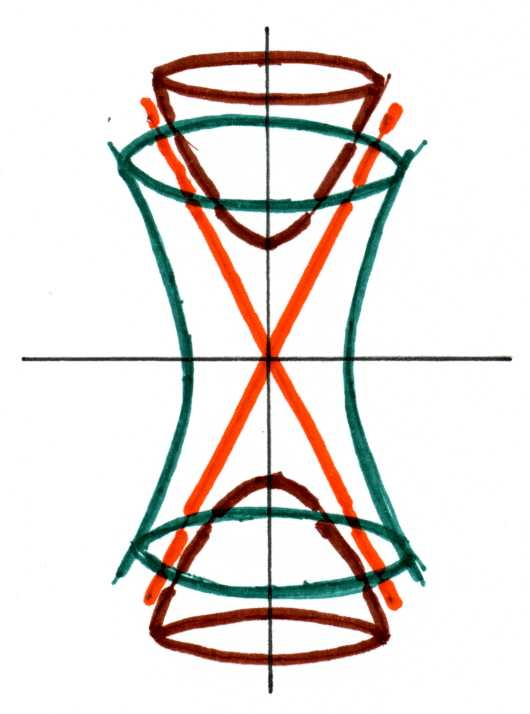
\includegraphics[width=\textwidth, height=5cm]{Pictures/LM.jpg}
	\end{subfigure}
	\caption{General Hyperboloid}
\end{figure}

Becaue of $\theta(p^0)$, Lorentz invariant measure is considered as integration on only positive $p^0$ surface of Lorentz Hyperboloid.

\VS

\textbf{* Why L.I Measure's name is L.I Measure?}

Consider Lorentz transform $p_3' = \gamma (p_3 + \beta E)\Com E' = \gamma(E+\beta p_3)$.

\begin{equation}
\begin{split}
 \delta^{(3)}(\vp - \vec{q}) &= \frac{\DT(\vp' - \vq')}{\abs{dp_3/dp_3'}} = \DT(\vp' - \vq')\OD[p_3'][p_3] = \DT(\vp'-\vq')\gamma\BKS{1+\beta\OD[E][p_3]}\\
 &= \DT(\vp'-\vq')\frac{\gamma}{E}(E+\beta p_3) = \DT(\vp'-\vq')\frac{E'}{E} \\
 &\therefore \Ep\DT(\vp - \vq) = E_{\vp}'\hs\DT(\vp'-\vq')
\end{split}
\end{equation}

Thus, $\Ep\DT(\vp-\vq)$ is Lorentz invariant. And therefore, $(2\pi)^3 2\Ep\DT(p-p') = \braket{p|p'}$ is Lorentz invariant.
\vs

\textbf{H.W.} Show that $\partial_0 \braket{u|v} = 0$
\newpage

\section*{Classical Field Theory}

Because of special relativity, we use the lagrangian density instead of usual lagrangian.

\begin{equation}
\begin{split}
  S &= \int dt \hs L = \int dt \int d^3x \L = \int d^4x \hs \L(\phi, \partial_\mu \phi) \\
  \delta S &= \int d^4x \BKS{\PD{\L}{\phi}\delta{\phi}+\PD{\L}{\partial_\mu\phi}\delta\partial_\mu\phi} = \int d^4x 
  \left[\BKS{\PD{\L}{\phi}-\partial_\mu\PD{\L}{\partial_\mu\phi}\delta\phi}+\partial_\mu\BKS{\PD{\L}{\partial_\mu\phi}\delta\phi}\right]=0 \\
  &\therefore \HS \PD{\L}{\phi} - \partial_\mu\PD{\L}{\partial_\mu\phi} = 0
\end{split}
\end{equation}

Then we can also obtain conjugate momentum density \& Hamiltonian density.

\begin{equation}
 \pi(x) = \PD{\L}{\partial_0 \phi(x)}\Com \hs \H(x) = \pi(x)\partial_0\phi(x) - \L \HS \HS (H = \int d^3x\hs\H)
\end{equation}

\HL

\section*{Lie Group}

Lie group is a group whose elements depend in a continuous \& differentiable way on a set of real parameters.
So, we can consider Lie group as \textit{Differentiable manifold.}

We took notation of Maggiore.
\begin{itemize}
 \item $g(\theta)$ : element of Lie group where $\theta^\alpha$ = real parameter.  (W.L.O.G $g(0)=e$)
 \item $D_R$ : Linear operator from Lie group to representation.
\end{itemize}

From definition of group \& these notations, we can get following properties.
\begin{enumerate}[i)]
 \item $D_R(e)=1$
 \item $D_R(g_1)D_R(g_2) = D_R(g_1g_2)$
\end{enumerate}

$*$ There is a property of a Lie group that is independent of the representation. - \textbf{Lie Algebra}

\VS

\subsection*{1. Generator}

Consider infinitesimal $\theta$. Then we can write unitary representation\footnotemark of this group as
$D_R(\theta) \simeq 1 + i\theta_aT^a_R$.
$\Rightarrow\hs T^a_R= -i \At{\PD{D_R}{\theta_a}}{\theta=0}$ \hs $T^a_R$ is called the generator of the representation
$D_R$ of group $g(\theta)$.

\footnotetext{$D_R(g(\theta)) = \exp{i\theta_aT^a_R}$}

\newpage

\subsection*{2. Lie Algebra}

Let $g_1, g_2$ be the elements of group $g$. Then if the group can be represented as unitary, we can write following reps.
\begin{equation}
 D_R(g_1) = e^{i\alpha_aT^a_R}\Com D_R(g_2) = e^{i\beta_aT^a_R}
\end{equation}

By properties of representation, we can get next equation.
\VS
\begin{equation}
 D_R(g_1)D_R(g_2) = D_R(g_1g_2) = D_R(g_1g_2) \hs\Rightarrow\hs e^{i\alpha_aT^a_R}e^{i\beta_aT^a_R} = e^{i\delta_aT^a_R}
\end{equation}

By BCH formula, for matrix $A, B$, \hs $e^A e^B = e^{A+B+\frac{1}{2}\Commutator[A][B]+\cdots}$.

\begin{equation}
\label{eq:21}
 \begin{split}
  &e^{i\alpha_aT^a_R}e^{i\beta_bT^b_R}=e^{i(\alpha_a+\beta_a)T^a_R - \frac{\alpha_a\beta_b}{2}\Commutator[T^a_R][T^b_R]}
  \equiv e^{i\delta_cT^c_R} \\
  \Rightarrow \hs &\alpha_a\beta_b\Commutator[T^a_R][T^b_R] = i\left[-2\{ \delta_c(\alpha,\beta) - \alpha_c - \beta_c \}\right]
 \end{split}
\end{equation}

It's easy to verify $\delta(\alpha,\beta)$ is linear for each $\alpha, \beta$. ($\delta_c(\alpha,0) = \alpha_c\Com \delta_c(0,\beta)=\beta_c)$
Thus, we can write $\delta_c$ as $\delta_c(\alpha,\beta) = \alpha_c + \beta_c + \tensor{C}{^a^b_c}\alpha_a\beta_b$ where $\tensor{C}{^{ab}_c}$
is constant. Thus, the last equation of \eqref{eq:21} becomes $\alpha_a\beta_b\Commutator[T^a_R][T^b_R] = i(-2\tensor{C}{^a^b_c}
\alpha_a\beta_b)T^c_R \equiv i\tensor{f}{^{ab}_c}\alpha_a\beta_bT^c_R$. Therefore we get the next relation.

\begin{equation}
 \therefore \Commutator[T^a][T^b] = i\tensor{f}{^a^b_c}T^c
\end{equation}

We called $\tensor{f}{^{ab}_c}$ as structure constant.

\vs

\begin{example}
\normalfont
 \begin{enumerate}
  \item $\tensor{f}{^{ij}_k}=\epsilon_{ijk}$ for SO(3), SU(2)
  \item $\tensor{f}{^{ab}_c}=0$ for abelian group. (This is the fundamental reason for why we can't quantize a charge of U(1).
 \end{enumerate}
\end{example}

\VS

\textbf{$*$ Non-Compact Groups have no unitary representations of finite dimensions}

: If a group is non-compact then to identify its generator we need infinite dimensional representations. (Hibert space of 1-particle state)

\newpage

\section*{Lorentz Group}

\subsection*{1. Rotation Group in 3D $-$ SO(3)}

Let $R$ be a representation of rotation and $r$ be a n-dimensional vector, then simply, 
$r \rightarrow r'=R\hs r$ where $R^TR=1$. Since $(R_1R_2)^T \ld R_1R_2 = R_2^T(R_1^TR_1)R_2 = 1$, it is closed of multiplication. And trivially identity \& inverse
are exist, $R$ forms a group. We called this group as O($n$). (In addition, if $\det R = 1$, then we call it SO($n$).)

\textbf{$*$ Generator}

\begin{align}
 R_z(\theta) = 
 \begin{pmatrix}
 \cos\theta & -\sin\theta  & 0 \\
 \sin\theta & \cos\theta & 0  \\
  0 & 0 & 0
 \end{pmatrix}
 \Rightarrow
 R_z(\delta \theta) =
 \begin{pmatrix}
  1 & -\delta\theta & 0 \\
  \delta\theta & 1 & 0 \\
  0 & 0 & 0
 \end{pmatrix}
 = 1 - i\delta\theta
 \begin{pmatrix}
  0 & -i & 0 \\
  i & 0 & 0 \\
  0 & 0 & 0
 \end{pmatrix}
 \equiv 1 - i\delta\theta J_z
\end{align}

Thus, we can find all of generators.

\begin{align}
 J_x = 
 \begin{pmatrix}
  0 & 0 & 0 \\
  0 & 0 & -i \\
  0 & i & 0
 \end{pmatrix}
 \Com \HS J_y  = 
 \begin{pmatrix}
  0 & 0 & i \\
  0 & 0 & 0 \\
  -i & 0 & 0 \\
 \end{pmatrix}
 \Com \HS J_z =
 \begin{pmatrix}
  0 & -i & 0 \\
  i & 0 & 0 \\
  0 & 0 & 0
 \end{pmatrix}
\end{align}

Then we can write unitary representation of Rotation group.

\begin{align}
 \therefore \hs\hs R(\theta) = e^{-i\vec{\theta}\ld \vec{J}} \HS \text{where} \hs \Commutator[J_i][J_j] = i\eps_{ijk}J_k
\end{align}

\VS

\subsection*{2. Unitary Group $-$ SU(2)}

Let $U$ be a representation of this group, then it shoud be satisfied $U^{\dagger}U = 1$. We called this group as
U($n$). (In addition, if $\det U = 1$, then we call it SU($n$).) Then $U$ can be written as below. (Check!)

\begin{align}
 U =
 \begin{pmatrix}
  a & b \\
  -b^* & a^*
 \end{pmatrix}
 \HS \text{where }\abs{a}^2 + \abs{b}^ 2 = 1 
\end{align}

We can take $a = e^{-i\alpha}\cos\gamma\Com b=e^{i\beta}\sin\gamma$, thus,

\begin{align}
\nonumber
 U(\delta) &=
 \begin{pmatrix}
  1-i\alpha & -\gamma-i\beta\gamma \\
  \gamma - i \beta\gamma & 1+i\alpha
 \end{pmatrix}
 \overset{\beta\gamma\rightarrow\beta}{\Longrightarrow} \alpha^2+\beta^2+\gamma^2 = 0 \\
 \Rightarrow \hs U(\delta) &= 1 - i\alpha\Pz -i\beta\Px -i\gamma\Py = 1 - i \eta \ld \frac{\vec{\sigma}}{2}
\end{align}

Since $\sigma$ is pauli matrices, it satisfy $\Commutator[\dfrac{\sigma^i}{2}][\dfrac{\sigma^j}{2}] = i\eps^{ijk}\dfrac{\sigma^k}{2}$
Thus, we can write 
\begin{equation}
\therefore \hs U(\eta) = e^{-i\eta\ld\frac{\sigma}{2}}
\end{equation}

\newpage

\subsection*{3. Lorentz Group}

We denote coordinates of Lorentz transformed frame by $x'$. Then we already knew  \newline $\tensor{x}{^{0'}}=\gamma(x^0+\beta x^i)\Com
\tensor{x}{^i^'}=\gamma(x^i+\beta x^0)$ where $\gamma^2 -\beta^2\gamma^2 = 1$. So, we can substitute 
$\gamma \equiv \cosh\eta\Com \gamma\beta \equiv \sinh \eta$ then $\tensor{x}{^\mu}' = \tensor{\Lambda}{^\mu_\nu}x^\nu$
where $\BKS{\tensor{\Lambda}{^\mu_\nu}}_x=
\begin{pmatrix}
 \cosh\eta & \sinh \eta & 0 & 0 \\
 \sinh\eta & \cosh \eta & 0 & 0 \\
 0 & 0 & 1 & 0 \\
 0 & 0 & 0 & 1
\end{pmatrix}$

For infinitesimal $\eta$, we can represent $\BKS{\tensor{\Lambda}{^\mu_\nu}}^i = 1- i\eta K^i$ where 

\begin{align}
 K_x = -i 
 \begin{pmatrix}
  0 & 1 & & \\
  1 & 0 & & \\
  & & &  \\
  & & & 
 \end{pmatrix}
 \Com K_y = - i
 \begin{pmatrix}
   0 & 0 & 1 & 0 \\
   0 & & & \\
   1 & & & \\
   0 & & &
 \end{pmatrix}
 \Com K_z = -i
 \begin{pmatrix}
  0 & 0 & 0 & 1 \\
  0 & & & \\
  0 & & & \\
  1 & & &
 \end{pmatrix}
\end{align}

\VS

For example, commutator of $K_x\Com K_y$ follows next relation.

\begin{align}
 \Commutator[K_x][K_y] =
 \begin{pmatrix}
  0 & 0 & 0 & 0 \\
  0 & 0 & -1 & 0 \\
  0 & 1 & 0 & 0 \\
  0 & 0 & 0 & 0
 \end{pmatrix}
 = 
 \begin{pmatrix}
  \hs & & & \\
  \hs & 0 & -1 & 0 \\
  \hs & 1 & 0 & 0 \\
  \hs & 0 & 0 & 0
 \end{pmatrix}
 = - i J_z \HS \text{(4D representation)}
\end{align}

\VS

So, pure Lorentz boost can't form a group $\Rightarrow$ They need rotation to form a group. \newline
We can obtain next commutation relation for $J\Com K$.

\begin{equation}
 \Commutator[J_i][J_j]=i\eps_{ijk}J_k\Com \Commutator[J_i][K_j] = i\eps_{ijk}K_k\Com \Commutator[K_i][K_j] = -i\eps_{ijk}J_k
\end{equation}

\VS

So, there are 3 Boost, 3 Rotation generators forming group. And we call this group as \textbf{Lorentz Group}.

Now, consider next two new generators.
\begin{equation}
 A = \frac{1}{2}(J+iK)\Com \hs B=\frac{1}{2}(J-iK)
\end{equation}

Then we can find the commutation relation.
\begin{equation}
 \Commutator[A_i][A_j] = i\eps_{ijk}A_k\Com\hs \Commutator[B_i][B_j]=i\eps_{ijk}B_k\Com\hs\Commutator[A_i][B_j]=0
\end{equation}

So, $A,B$ obey SU($2$) algebra. Thus the Lorentz group is isomorphic to SU($2$)$\otimes$SU($2$). Therefore we can label
the angular momentum of Lorentz group as $(2j_+ + 1\Com 2j_- + 1)$

\newpage

\subsection*{4. Decomposition of Lorentz tensors under SO($3$)}

Let $j$ be the angular momentum of tensor representation of SO($3$). For $j$, dimension of the representation is $2j+1$. ($j$ is integer) 
Then let notice some representations which have different angular momentum.
\begin{itemize}
 \item $j = 0$: dim = 0 $\rightarrow$ Scalar
 \item $j = 1$: dim = 3 $\rightarrow$ Spartial vector
\end{itemize}
For convenience, let $\phi$ be a scalar then we describe this as $\phi \in \mathbf{0}$. Also, let $V^i$ be a spartial vector then we describe it as $V^i \in \mathbf{1}$.

Now, consider 4-vector. $x^\mu = (x^0, x^i)$ where $x^0 \in \mathbf{0}\Com x^i \in \mathbf{1}$. Thus, we write this as $x^\mu \in \mathbf{0} \oplus \mathbf{1}$.
Then let consider the angular momentum of generic tensor $\tensor{T}{^\mu ^\nu}$.

\begin{equation}
 \tensor{T}{^\mu ^\nu} \in (\mathbf{0}\oplus\mathbf{1})\otimes(\mathbf{0}\oplus\mathbf{1}) = (\mathbf{0}\otimes\mathbf{0})\oplus(\mathbf{0}\otimes\mathbf{1})
 \oplus(\mathbf{1}\otimes\mathbf{0})\oplus(\mathbf{1}\otimes\mathbf{1}) = \mathbf{0}\oplus\mathbf{1}\oplus\mathbf{1}\oplus(\mathbf{0}\oplus\mathbf{1}\oplus\mathbf{2})
 \footnotemark[1]
\end{equation}

\footnotetext[1]{For $(j_1,j_2)$, we can obtain total angular momentum by counting angular momentums between $\abs{j_1 - j_2}\Com j_1+j_2$. \newline
For example, $\mathbf{0}\otimes\mathbf{0} = 0\Com \mathbf{0}\otimes\mathbf{1} = 1\Com \mathbf{1}\otimes\mathbf{1} = \mathbf{0}\oplus\mathbf{1}\oplus\mathbf{2}$}

\vs

This result means, the generic tensor $\tensor{T}{^\mu ^\nu}$ can be decomposed by 1 scalar, 2 spartial vectors and the tensor which has 9 degrees of freedom.
(dimension of $\mathbf{0}\oplus\mathbf{1}\oplus\mathbf{2}$ is $1 + 3 + 5 = 9$). And it's easy to find what kinds of these elements are - trace, anti-symmetric tensor ($A^{\mu\nu}$)
and traceless symmetric tensor ($S^{\mu\nu}$).

\begin{itemize}
 \item $tr(T) \in \mathbf{0}$
 \item $\tensor{A}{^\mu ^\nu}$ : six components. $\tensor{A}{^0 ^i}, \frac{1}{2}\eps_{ijk}\tensor{A}{^j ^k}$ are spartial vectors. $\Rightarrow \hs \tensor{A}{^\mu ^\nu} \in
 \mathbf{1}\oplus\mathbf{1}$
 \item $\tensor{S}{^\mu ^\nu}$ : dimension of $S^{\mu\nu}$ is $(4-1)+6 = 9$ (4 is diagonal, -1 is traceless, 6 is symmetric components)
\end{itemize}

\vs

Therefore we can decompose the second rank generic tensor as trace, anti-symmetric tensor and traceless symmetric tensor.

\vs

\textbf{$*$ How to represent spinor as above notation?}

: we know SU($2$) has same algebra with SO($3$).\footnotemark[2]
\footnotetext[2]{We explain this issue at appendix A}
So, spinor also has angular momentum $j$ but it is half integer. For $j=\frac{1}{2}$, dimension is 2 and $J^i = \frac{\sigma^i}{2}$ where $\sigma^i$ is pauli matrices.

Since $\mathbf{\frac{1}{2}}\otimes\mathbf{0} = \mathbf{0}\otimes\mathbf{\frac{1}{2}} = \mathbf{\frac{1}{2}}\Com \hs \mathbf{\frac{1}{2}}\otimes\mathbf{\frac{1}{2}} = 
\mathbf{0}\oplus\mathbf{1}$, we can find SU($2$)$\otimes$SU($2$) = SO($1$,$3$).

\newpage

\subsection*{5. Lorentz Algebra}

\subsubsection*{1) Scalar Representation}

Since $\vec{L} = \vec{x} \times \vec{p}$, for Quantum mechanically, we can write $L^{ij} = -i(x^i\nabla^j - x^j\nabla^i)$. Then for spacetime, we can write
$L^{\mu\nu} = i(x^\mu\partial^\nu - x^\nu\partial^\mu)$. We call it as scalar representation of Lorentz group. Trivially, $L^{\mu\nu}$ is antisymmetric. So, 
there are 6 degrees of freedom: $L^{0i} =$ boost, $L^{ij} =$ rotation. And we can find next commutation relation.
\footnotetext[0]{All proofs of commutation relation of representations are noted at appendix.}

\begin{equation}
 \Commutator[L^{\mu\nu}][L^{\rho\sigma}] = -i(\eta^{\mu\rho}L^{\nu\sigma}-\eta^{\mu\sigma}L^{\nu\rho} - \eta^{\nu\rho}L^{\mu\sigma} +\eta^{\nu\sigma}L^{\mu\rho})
\end{equation}

\VS

We call it as commutation rule of Lorentz algebra. Then any matrices that are represent this algebra must obey same commutation rules.

\subsubsection*{2) Vector Representation}

Consider $\tensor{\BKS{\J{\mu\nu}}}{^\alpha _\beta} = i(\eta^{\mu\alpha}\delta^\nu_\beta - \eta^{\nu\alpha}\delta^\mu_\beta)$. \footnotemark[1]
\footnotetext[1]{$\mu,\nu$ represent 6 matrices and $\alpha, \beta$ represent components}
Then we can check $\J{\mu\nu}$ also satisfies the commutation rule of Lorentz algebra. So, $\J{\mu\nu}$ are also representations of Lorentz group.
We call it as the vector representation of Lorentz group. Because we wrote the Lorentz transform of 4-vector as 

\begin{equation}
 V^\alpha \hs \rightarrow \hs \BKS{\delta^\alpha_\beta - \frac{i}{2}\omega_{\mu\nu}\tensor{\BKS{\J{\mu\nu}}}{^\alpha _\beta}}V^\beta \equiv \tensor{\Lambda}{^\alpha _\beta}V^\beta
\end{equation}

\VS

where $\omega_{\mu\nu}$ is anti-symmetric variable. And we can find $\J{0i}$ are boosts and $\J{ij}$ are rotations where $\omega_{0i} = \beta\Com \omega_{ij} = \theta$.
(It's easy to find. If you have some troubles to deal this, then see Peskin \& Schroeder.)
\subsubsection*{3) Spinor Representation}

Consider $S^{\mu\nu} = \dfrac{i}{4}\Commutator[\gamma^\mu][\gamma^\nu]$ where $\ACommutator{\gamma^\mu}{\gamma^\nu} = 2g^{\mu\nu}$. Then it is also generator of Lorentz group.
Thus, $1-\frac{i}{2}\omega_{\rho\sigma}S^{\rho\sigma}$ is also representation of Lorentz transform. We call it \textbf{Spinor Representation} and
denote it by $\Lambda_{\frac{1}{2}}$.

We can find next relations:
\begin{itemize}
 \item Boost : $S^{0j} = \tfrac{i}{4}\Commutator[\gamma^{0}][\gamma^{i}]=-\frac{i}{2}
     \begin{pmatrix}
         \sigma^i & 0 \\
         0 & -\sigma^{i}
     \end{pmatrix}$
 \item Rotation : $S^{ij} = \tfrac{i}{4}\Commutator[\gamma^{i}][\gamma^{j}]=\frac{1}{2}\epsilon^{ijk}
     \begin{pmatrix}
         \sigma^{k} & 0 \\
         0 & \sigma^{k}
     \end{pmatrix}
     \equiv \tfrac{1}{2}\epsilon^{ijk}\Sigma^{k}$
\end{itemize}








%------------------------------------------------------------------------------------------------------------------------------------------------------------------------
\newpage
\appendix

\section{SU($2$) \& O($3$)}

Consider two component spinor $\xi =
\begin{pmatrix}
 \xi_1 \\
 \xi_2
\end{pmatrix}$
which is transformed by $ U =
\begin{pmatrix}
 a & b \\
 -b^* & a^* 
\end{pmatrix}
\Com \abs{a}^2 + \abs{b}^2 = 1$. \newline
Since $\xi \rightarrow U\xi\Com \xi^{\dagger} \rightarrow \xi^{\dagger}U^{\dagger}$, we can find $\xi^{\dagger}\xi = \abs{\xi_1}^2+\abs{\xi_2}^2 $ is invariant under $U$.
Now, consider transformation of this spinor by specific components.

\begin{align}
\nonumber
&\begin{pmatrix}
  \xi_1 \\
  \xi_2
 \end{pmatrix}
 \rightarrow
 \begin{pmatrix}
  \xi_1' \\
  \xi_2'
 \end{pmatrix}
 =
 \begin{pmatrix}
  a\xi_1 + b\xi_2 \\
  -b^*\xi_1 + a^*\xi_2
 \end{pmatrix}
 \Com
 \begin{pmatrix}
  \tensor{\xi}{_1 ^*}' & \tensor{\xi}{_2 ^*}' 
 \end{pmatrix}
 =
 \begin{pmatrix}
  \xi_1^* & \xi_2^*
 \end{pmatrix}
 \begin{pmatrix}
  a^* & -b \\
  b^* & a
 \end{pmatrix}
 =
 \begin{pmatrix}
  a^*\xi_1^* + b^*\xi_2^* & -b\xi_1^* + a\xi_2^*
 \end{pmatrix} \\
 \Rightarrow &
 \begin{pmatrix}
  \tensor{\xi}{_1 ^*}' \\
  \tensor{\xi}{_2 ^*}' 
 \end{pmatrix}
 =
 \begin{pmatrix}
  a^* & b^* \\
  -b & a
 \end{pmatrix}
 \begin{pmatrix}
  \xi_1^* \\
  \xi_2^*
 \end{pmatrix}
 \hs \Rightarrow \hs 
 \begin{pmatrix}
  -\tensor{\xi}{_2 ^*}' \\
  \tensor{\xi}{_1 ^*}'
 \end{pmatrix}
 = U
 \begin{pmatrix}
  -\xi_2^* \\
  \xi_1^*
 \end{pmatrix}
\end{align}

Thus, $ \xi = 
\begin{pmatrix}
 \xi_1 \\
 \xi_2
\end{pmatrix}
\Com \tilde{\xi} = 
\begin{pmatrix}
 -\xi_2^* \\
 \xi_1^*
\end{pmatrix}$
are states which are transformed by $U$.\footnotemark[1]
\footnotetext[1]{This procedure is called as \textit{Flip Spin} $\tilde{\xi} = -i\sigma_2\xi^*$}
So, we can guess there is some relationship between $\xi$ and $\tilde{\xi}$. We denote it $\sim$. Then now consider $\xi^{\dagger}$.

\begin{align}
 \xi^{\dagger} \sim \BKS{\tilde{\xi}}^\dagger =
 \begin{pmatrix}
  -\xi_2 & \xi_1
 \end{pmatrix}
 \hs \Rightarrow \hs \xi \xi^{\dagger} \sim
 \begin{pmatrix}
  \xi_1 \\
  \xi_2
 \end{pmatrix}
 \begin{pmatrix}
  -\xi_2 & \xi_1
 \end{pmatrix}
 =
 \begin{pmatrix}
  -\xi_1 \xi_2 & \xi_1^2 \\
  -\xi_2^2 & \xi_2 \xi_1
 \end{pmatrix}
 \equiv h
\end{align}

We know $\xi \xi^\dagger \rightarrow U\xi\xi^{\dagger}U^{\dagger}\Rightarrow h \rightarrow UhU^{\dagger}$, thus, we can find $\det{h} = \det{h'}$.
Let $h = \vec{\sigma}\ld\vec{r}$ where $\vec{r} = (x,y,z)$, $\vec{\sigma}$ are pauli matrices. \footnotemark[2] 
\footnotetext[2]{It is position vector in SU($2$)}
Then 

\begin{align}
 h = 
 \begin{pmatrix}
  z & x - iy \\
  x + iy & -z
 \end{pmatrix}
 \Rightarrow z = -\xi_1\xi_2 \Com x = \frac{1}{2}\BKS{\xi_1^2 - \xi_2^2} \Com y = \frac{-1}{2i}\BKS{\xi_1^2 + \xi_2^2}
\end{align}

We know $\det{h}$ is invariant under this transformation, thus, $\det{h} = -(x^2 + y^2 + z^2)$ is invariant. $\Rightarrow$ O($3$) Transform!

{\centering
$\therefore$ An SU($2$) transformation on $
\begin{pmatrix}
 \xi_1 \\
 \xi_2
\end{pmatrix}$
 = O($3$) transformation on $
\begin{pmatrix}
 x \\
 y \\
 z
\end{pmatrix}$

\begin{equation}
 \therefore U(\eta) = e^{-i\vec{\eta}\cdot\frac{\vec{\sigma}}{2}} \hs \longleftrightarrow \hs R(\theta) = e^{-i\vec{\theta}\ld \vec{J}}
\end{equation}}


Therefore we can conclude the rotation generator of spinor is $\vec{J} = \dfrac{\vec{\sigma}}{2}$.

\newpage

\section{SL(2, $\mathbb{C}$)}

Consider the next transform for $X = x_\mu \sigma^\mu$ ($\sigma^{\mu} = (1, \vec{\sigma}))$: 

\begin{equation}
 X \rightarrow X' = SXS^{\dagger}
\end{equation}

\vs

If $S\in SL(2,\mathbb{C})$, then this transform describes the Lorentz transformation.

\VS

\textbf{Proof :}

\begin{quote}

The definition of $SL(2,\mathbb{C})$ is \hs $\forall A \in SL(2,\mathbb{C})\Com A_{ij} \in \mathbb{C} \hs \& \hs \det{A} = 1$.
So, this transform preserves determinant (Symmetric Transform). Then let consider $\det{X}$.

\begin{align}
 X &= x_\mu \sigma^{\mu} = x^0 \cdot 1 - x^1 \sigma^1 - x^2 \sigma^2 -x^3 \sigma^3 \\
    &= x^0 \Id - x^1 \Px - x^2 \Py -x^3\Pz \\
    &=
    \begin{pmatrix}
     x^0 - x^3 & -x^1 - ix^2 \\
     -x^1 + ix^2 & x^0 + x^3
    \end{pmatrix} \\
 \therefore \det{X} &= (x^0)^2 - (x^1)^2 - (x^2)^2 - (x^3)^2 = x^2
\end{align} 

\VS

Since the transform preserves determinant, we can get next relation.

\begin{equation}
 x'^2 = x^2
\end{equation}

\vs

which is same as Lorentz transform.
\end{quote}

\vs

Now, let find matrix elements of Lorentz transform on this representation.

First, let's see next lemma

\begin{lemma}
   $ x\UP\mu = \frac{1}{2}tr(\bar{\sigma}\UP\mu x_\nu \sigma\UP\nu)$
\end{lemma}

\xymatrix{
  & A \ar[d] \\
  B \ar[ur] \ar[r] & C}

\end{document}